\section{Introduction}
\label{sec:Introduction}

In this lab course data from the ATLAS experiment at the LHC is used to search for new particles decaying to a top quark and an anti-top quark. As an extension of the Standard Model of particle physics, a resonance is predicted that might be such a new particle. In the Standard Model of particle physics the top quark is the most massive elementary particle known to date. It can be produced in $p\bar{p}$ collisions. In most cases a $t\bar{t}$ pair is produced via the strong interaction. The $t\bar{t}$ pair decays via the weak interaction to a $W$ boson and a down-type quark, where the down-type quark usually is a bottom-quark $b$. The $W$ boson can either decay into a lepton and a neutrino or into a pair of quarks: $W^+ \rightarrow l^+ \nu_l, W^+ \rightarrow u\bar{d}$ or $W^+ \rightarrow c\bar{s}$.

The quarks in the decay hadronize and form jets of color neutral products. The channel in which both $W$ bosons decay to a lepton and its corresponding neutrino is called the \emph{dilepton channel}, whereas the channel in which both $W$ bosons decay hadronically is called the \emph{all-hadronic channel}. The channel in which one $W$ boson decays leptonically and the other decays hadronically is called the \emph{lepton+jets channel}.

\begin{figure}[H]
  \centering
  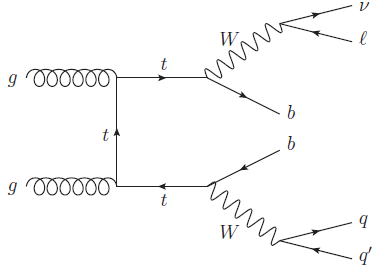
\includegraphics[width=0.4\textwidth]{graphics/decay.png}
  \caption{Feynman diagram of top quark production and the following decay to a \emph{lepton+jets channel}.}
  \label{fig:decay}
\end{figure}

Since there is much background in the \emph{all-hadronic channel}, the \emph{lepton+jets channel} is preferred for use in top-quark analyses. The \emph{dilepton channel} has very little branching fractions. The decay particles can be registered in a detector and are reconstructed by algorithms which use the different signatures left by the particles that propagated through the detector. To distinguish events with top quarks in the final state from background events, the missing transverse momentum is used to determine whether a neutrino has been produced. This is the case for the \emph{lepton+jets channel}.
Jets originating from other quarks than a $b$-quark are distinguished by identifying a $B$-hadron within the $b$-jets.

First, to search for a hypothetical massive $Z'$ boson decaying to top quarks, the size of the dataset is reduced. By event selection the signal-to-background ratio is increased. To model the background spectrum Monte Carlo simulations are used. MC simulations and data are then compared to check the validity of the simulations. A final discriminant is chosen and is used in a statistical analysis to determine the amount of signal on top of the background distribution.
